\documentclass[1p]{elsarticle_modified}
%\bibliographystyle{elsarticle-num}

%\usepackage[colorlinks]{hyperref}
%\usepackage{abbrmath_seonhwa} %\Abb, \Ascr, \Acal ,\Abf, \Afrak
\usepackage{amsfonts}
\usepackage{amssymb}
\usepackage{amsmath}
\usepackage{amsthm}
\usepackage{scalefnt}
\usepackage{amsbsy}
\usepackage{kotex}
\usepackage{caption}
\usepackage{subfig}
\usepackage{color}
\usepackage{graphicx}
\usepackage{xcolor} %% white, black, red, green, blue, cyan, magenta, yellow
\usepackage{float}
\usepackage{setspace}
\usepackage{hyperref}

\usepackage{tikz}
\usetikzlibrary{arrows}

\usepackage{multirow}
\usepackage{array} % fixed length table
\usepackage{hhline}

%%%%%%%%%%%%%%%%%%%%%
\makeatletter
\renewcommand*\env@matrix[1][\arraystretch]{%
	\edef\arraystretch{#1}%
	\hskip -\arraycolsep
	\let\@ifnextchar\new@ifnextchar
	\array{*\c@MaxMatrixCols c}}
\makeatother %https://tex.stackexchange.com/questions/14071/how-can-i-increase-the-line-spacing-in-a-matrix
%%%%%%%%%%%%%%%

\usepackage[normalem]{ulem}

\newcommand{\msout}[1]{\ifmmode\text{\sout{\ensuremath{#1}}}\else\sout{#1}\fi}
%SOURCE: \msout is \stkout macro in https://tex.stackexchange.com/questions/20609/strikeout-in-math-mode

\newcommand{\cancel}[1]{
	\ifmmode
	{\color{red}\msout{#1}}
	\else
	{\color{red}\sout{#1}}
	\fi
}

\newcommand{\add}[1]{
	{\color{blue}\uwave{#1}}
}

\newcommand{\replace}[2]{
	\ifmmode
	{\color{red}\msout{#1}}{\color{blue}\uwave{#2}}
	\else
	{\color{red}\sout{#1}}{\color{blue}\uwave{#2}}
	\fi
}

\newcommand{\Sol}{\mathcal{S}} %segment
\newcommand{\D}{D} %diagram
\newcommand{\A}{\mathcal{A}} %arc


%%%%%%%%%%%%%%%%%%%%%%%%%%%%%5 test

\def\sl{\operatorname{\textup{SL}}(2,\Cbb)}
\def\psl{\operatorname{\textup{PSL}}(2,\Cbb)}
\def\quan{\mkern 1mu \triangleright \mkern 1mu}

\theoremstyle{definition}
\newtheorem{thm}{Theorem}[section]
\newtheorem{prop}[thm]{Proposition}
\newtheorem{lem}[thm]{Lemma}
\newtheorem{ques}[thm]{Question}
\newtheorem{cor}[thm]{Corollary}
\newtheorem{defn}[thm]{Definition}
\newtheorem{exam}[thm]{Example}
\newtheorem{rmk}[thm]{Remark}
\newtheorem{alg}[thm]{Algorithm}

\newcommand{\I}{\sqrt{-1}}
\begin{document}

%\begin{frontmatter}
%
%\title{Boundary parabolic representations of knots up to 8 crossings}
%
%%% Group authors per affiliation:
%\author{Yunhi Cho} 
%\address{Department of Mathematics, University of Seoul, Seoul, Korea}
%\ead{yhcho@uos.ac.kr}
%
%
%\author{Seonhwa Kim} %\fnref{s_kim}}
%\address{Center for Geometry and Physics, Institute for Basic Science, Pohang, 37673, Korea}
%\ead{ryeona17@ibs.re.kr}
%
%\author{Hyuk Kim}
%\address{Department of Mathematical Sciences, Seoul National University, Seoul 08826, Korea}
%\ead{hyukkim@snu.ac.kr}
%
%\author{Seokbeom Yoon}
%\address{Department of Mathematical Sciences, Seoul National University, Seoul, 08826,  Korea}
%\ead{sbyoon15@snu.ac.kr}
%
%\begin{abstract}
%We find all boundary parabolic representation of knots up to 8 crossings.
%
%\end{abstract}
%\begin{keyword}
%    \MSC[2010] 57M25 
%\end{keyword}
%
%\end{frontmatter}

%\linenumbers
%\tableofcontents
%
\newcommand\colored[1]{\textcolor{white}{\rule[-0.35ex]{0.8em}{1.4ex}}\kern-0.8em\color{red} #1}%
%\newcommand\colored[1]{\textcolor{white}{ #1}\kern-2.17ex	\textcolor{white}{ #1}\kern-1.81ex	\textcolor{white}{ #1}\kern-2.15ex\color{red}#1	}

{\Large $\underline{12a_{0049}~(K12a_{0049})}$}

\setlength{\tabcolsep}{10pt}
\renewcommand{\arraystretch}{1.6}
\vspace{1cm}\begin{tabular}{m{100pt}>{\centering\arraybackslash}m{274pt}}
\multirow{5}{120pt}{
	\centering
	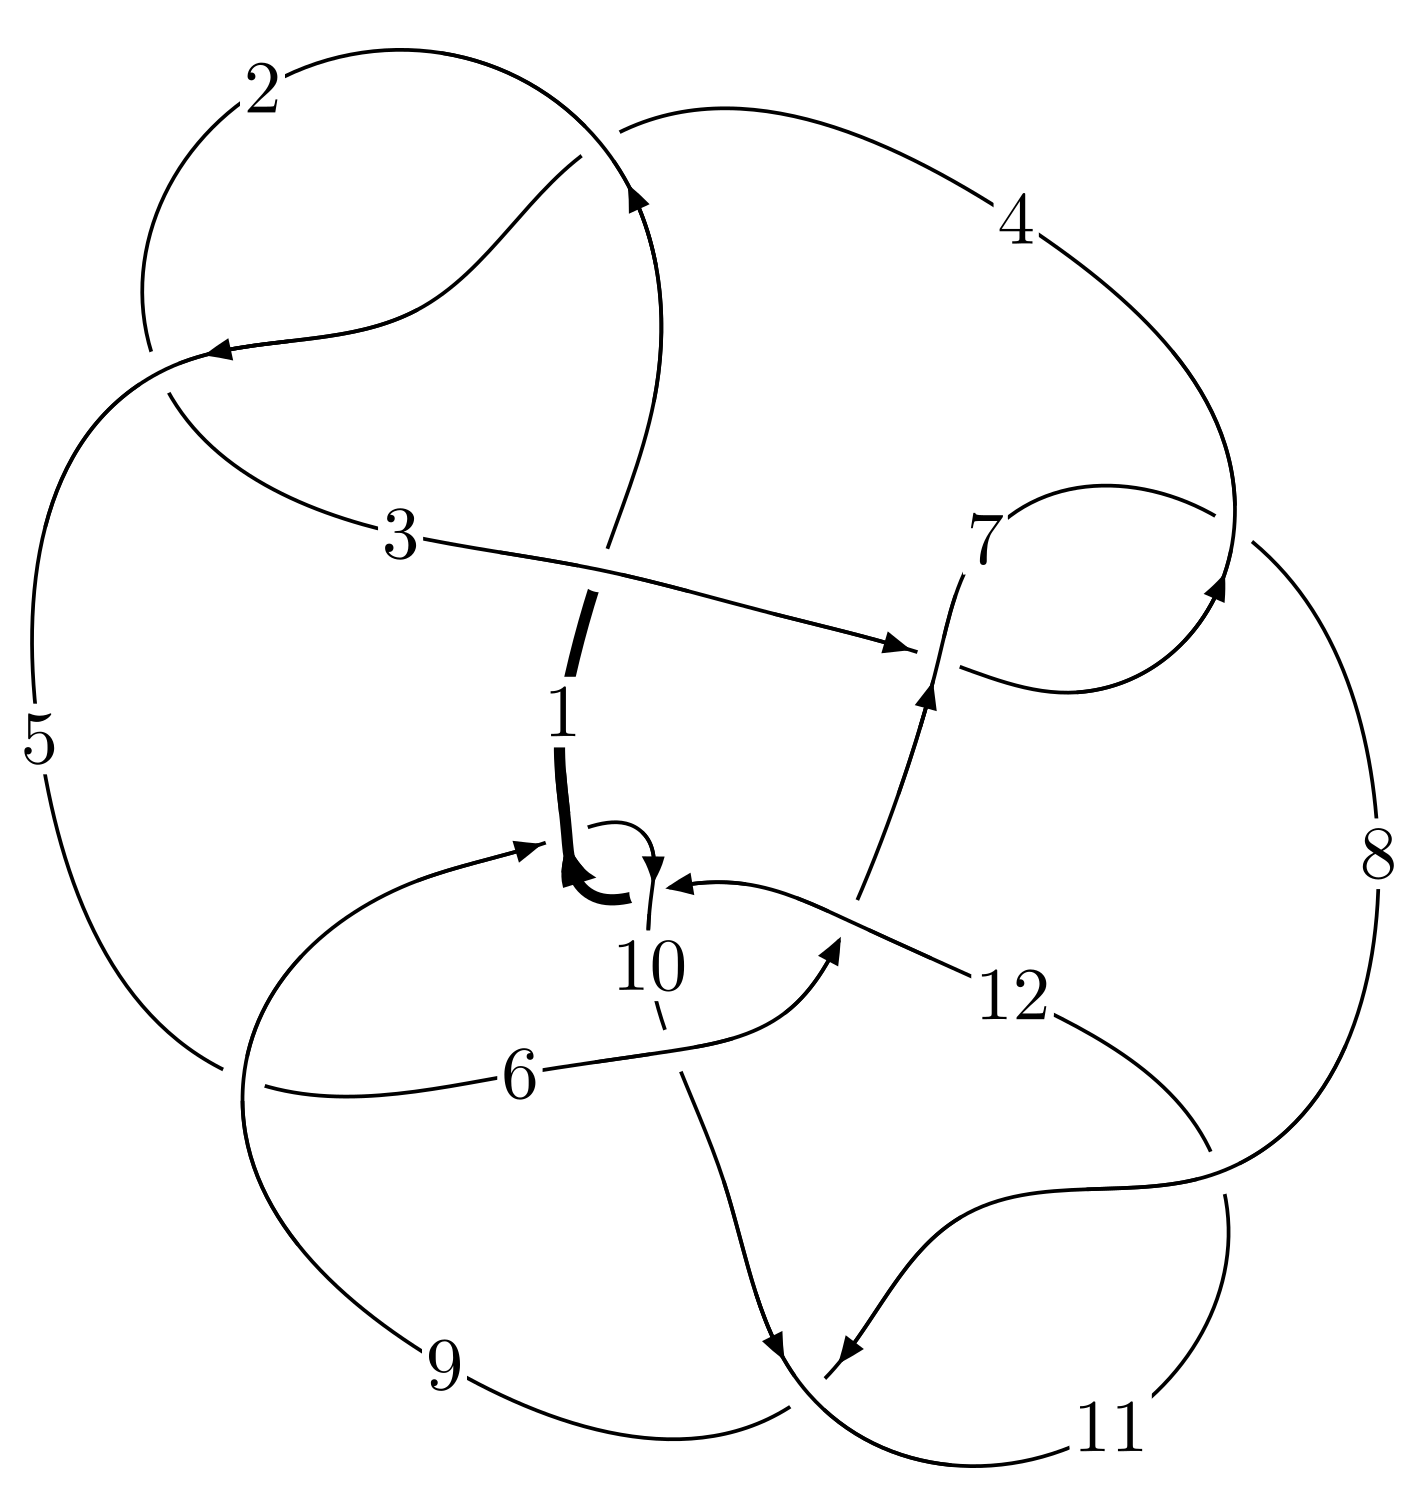
\includegraphics[width=112pt]{../../../GIT/diagram.site/Diagrams/png/850_12a_0049.png}\\
\ \ \ A knot diagram\footnotemark}&
\allowdisplaybreaks
\textbf{Linearized knot diagam} \\
\cline{2-2}
 &
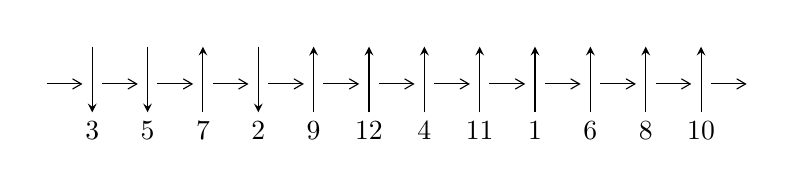
\begin{tikzpicture}[x=20pt, y=17pt]
	% nodes
	\node (C0) at (0, 0) {};
	\node (C1) at (1, 0) {};
	\node (C1U) at (1, +1) {};
	\node (C1D) at (1, -1) {3};

	\node (C2) at (2, 0) {};
	\node (C2U) at (2, +1) {};
	\node (C2D) at (2, -1) {5};

	\node (C3) at (3, 0) {};
	\node (C3U) at (3, +1) {};
	\node (C3D) at (3, -1) {7};

	\node (C4) at (4, 0) {};
	\node (C4U) at (4, +1) {};
	\node (C4D) at (4, -1) {2};

	\node (C5) at (5, 0) {};
	\node (C5U) at (5, +1) {};
	\node (C5D) at (5, -1) {9};

	\node (C6) at (6, 0) {};
	\node (C6U) at (6, +1) {};
	\node (C6D) at (6, -1) {12};

	\node (C7) at (7, 0) {};
	\node (C7U) at (7, +1) {};
	\node (C7D) at (7, -1) {4};

	\node (C8) at (8, 0) {};
	\node (C8U) at (8, +1) {};
	\node (C8D) at (8, -1) {11};

	\node (C9) at (9, 0) {};
	\node (C9U) at (9, +1) {};
	\node (C9D) at (9, -1) {1};

	\node (C10) at (10, 0) {};
	\node (C10U) at (10, +1) {};
	\node (C10D) at (10, -1) {6};

	\node (C11) at (11, 0) {};
	\node (C11U) at (11, +1) {};
	\node (C11D) at (11, -1) {8};

	\node (C12) at (12, 0) {};
	\node (C12U) at (12, +1) {};
	\node (C12D) at (12, -1) {10};
	\node (C13) at (13, 0) {};

	% arrows
	\draw[->,>={angle 60}]
	(C0) edge (C1) (C1) edge (C2) (C2) edge (C3) (C3) edge (C4) (C4) edge (C5) (C5) edge (C6) (C6) edge (C7) (C7) edge (C8) (C8) edge (C9) (C9) edge (C10) (C10) edge (C11) (C11) edge (C12) (C12) edge (C13) ;	\draw[->,>=stealth]
	(C1U) edge (C1D) (C2U) edge (C2D) (C3D) edge (C3U) (C4U) edge (C4D) (C5D) edge (C5U) (C6D) edge (C6U) (C7D) edge (C7U) (C8D) edge (C8U) (C9D) edge (C9U) (C10D) edge (C10U) (C11D) edge (C11U) (C12D) edge (C12U) ;
	\end{tikzpicture} \\
\hhline{~~} \\& 
\textbf{Solving Sequence} \\ \cline{2-2} 
 &
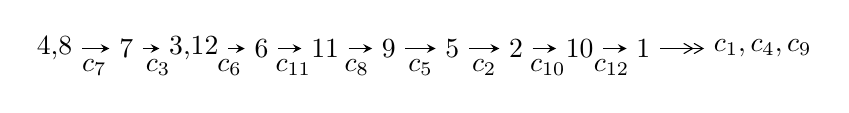
\begin{tikzpicture}[x=23pt, y=7pt]
	% node
	\node (A0) at (-1/8, 0) {4,8};
	\node (A1) at (1, 0) {7};
	\node (A2) at (33/16, 0) {3,12};
	\node (A3) at (25/8, 0) {6};
	\node (A4) at (33/8, 0) {11};
	\node (A5) at (41/8, 0) {9};
	\node (A6) at (49/8, 0) {5};
	\node (A7) at (57/8, 0) {2};
	\node (A8) at (65/8, 0) {10};
	\node (A9) at (73/8, 0) {1};
	\node (C1) at (1/2, -1) {$c_{7}$};
	\node (C2) at (3/2, -1) {$c_{3}$};
	\node (C3) at (21/8, -1) {$c_{6}$};
	\node (C4) at (29/8, -1) {$c_{11}$};
	\node (C5) at (37/8, -1) {$c_{8}$};
	\node (C6) at (45/8, -1) {$c_{5}$};
	\node (C7) at (53/8, -1) {$c_{2}$};
	\node (C8) at (61/8, -1) {$c_{10}$};
	\node (C9) at (69/8, -1) {$c_{12}$};
	\node (A10) at (11, 0) {$c_{1},c_{4},c_{9}$};

	% edge
	\draw[->,>=stealth]	
	(A0) edge (A1) (A1) edge (A2) (A2) edge (A3) (A3) edge (A4) (A4) edge (A5) (A5) edge (A6) (A6) edge (A7) (A7) edge (A8) (A8) edge (A9) ;
	\draw[->>,>={angle 60}]	
	(A9) edge (A10);
\end{tikzpicture} \\ 

\end{tabular} \\

\footnotetext{
The image of knot diagram is generated by the software ``\textbf{Draw programme}" developed by Andrew Bartholomew(\url{http://www.layer8.co.uk/maths/draw/index.htm\#Running-draw}), where we modified some parts for our purpose(\url{https://github.com/CATsTAILs/LinksPainter}).
}\phantom \\ \newline 
\centering \textbf{Ideals for irreducible components\footnotemark of $X_{\text{par}}$} 
 
\begin{align*}
I^u_{1}&=\langle 
2.20260\times10^{103} u^{47}+1.71175\times10^{103} u^{46}+\cdots+6.39981\times10^{106} b-1.52221\times10^{105},\\
\phantom{I^u_{1}}&\phantom{= \langle  }3.79806\times10^{106} u^{47}+1.55054\times10^{106} u^{46}+\cdots+1.02397\times10^{108} a-1.21535\times10^{109},\\
\phantom{I^u_{1}}&\phantom{= \langle  }u^{48}-9 u^{46}+\cdots-688 u+128\rangle \\
I^u_{2}&=\langle 
-1.12143\times10^{21} a u^{39}-8.51510\times10^{20} u^{39}+\cdots+5.02212\times10^{21} a-6.07964\times10^{21},\\
\phantom{I^u_{2}}&\phantom{= \langle  }1.50092\times10^{21} a u^{39}+7.38054\times10^{22} u^{39}+\cdots+1.98528\times10^{22} a+5.64927\times10^{23},\;u^{40}- u^{39}+\cdots+8 u+4\rangle \\
I^u_{3}&=\langle 
b+1,\;2 u^5-4 u^3-2 u^2+2 a+4 u+3,\;u^6+u^5- u^4-2 u^3+u+1\rangle \\
\\
I^v_{1}&=\langle 
a,\;-20 v^2+13 b+69 v-1,\;4 v^3-13 v^2- v-1\rangle \\
I^v_{2}&=\langle 
a,\;b^2- b v- b+v+1,\;v^2+v+1\rangle \\
\end{align*}
\raggedright * 5 irreducible components of $\dim_{\mathbb{C}}=0$, with total 141 representations.\\
\footnotetext{All coefficients of polynomials are rational numbers. But the coefficients are sometimes approximated in decimal forms when there is not enough margin.}
\newpage
\renewcommand{\arraystretch}{1}
\centering \section*{I. $I^u_{1}= \langle 2.20\times10^{103} u^{47}+1.71\times10^{103} u^{46}+\cdots+6.40\times10^{106} b-1.52\times10^{105},\;3.80\times10^{106} u^{47}+1.55\times10^{106} u^{46}+\cdots+1.02\times10^{108} a-1.22\times10^{109},\;u^{48}-9 u^{46}+\cdots-688 u+128 \rangle$}
\flushleft \textbf{(i) Arc colorings}\\
\begin{tabular}{m{7pt} m{180pt} m{7pt} m{180pt} }
\flushright $a_{4}=$&$\begin{pmatrix}0\\u\end{pmatrix}$ \\
\flushright $a_{8}=$&$\begin{pmatrix}1\\0\end{pmatrix}$ \\
\flushright $a_{7}=$&$\begin{pmatrix}1\\u^2\end{pmatrix}$ \\
\flushright $a_{3}=$&$\begin{pmatrix}- u\\- u^3+u\end{pmatrix}$ \\
\flushright $a_{12}=$&$\begin{pmatrix}-0.0370915 u^{47}-0.0151424 u^{46}+\cdots-33.2399 u+11.8690\\-0.000344167 u^{47}-0.000267469 u^{46}+\cdots-1.40675 u+0.0237852\end{pmatrix}$ \\
\flushright $a_{6}=$&$\begin{pmatrix}-0.0117969 u^{47}-0.00536501 u^{46}+\cdots-11.1030 u+4.23953\\-0.00240170 u^{47}+0.000899905 u^{46}+\cdots-1.74418 u+0.851220\end{pmatrix}$ \\
\flushright $a_{11}=$&$\begin{pmatrix}-0.0367474 u^{47}-0.0148750 u^{46}+\cdots-31.8331 u+11.8452\\-0.000344167 u^{47}-0.000267469 u^{46}+\cdots-1.40675 u+0.0237852\end{pmatrix}$ \\
\flushright $a_{9}=$&$\begin{pmatrix}-0.0214507 u^{47}-0.00655382 u^{46}+\cdots-18.8650 u+7.82073\\-0.00136402 u^{47}-0.00245258 u^{46}+\cdots-1.53193 u+0.301599\end{pmatrix}$ \\
\flushright $a_{5}=$&$\begin{pmatrix}-0.0154147 u^{47}-0.00689804 u^{46}+\cdots-13.6620 u+4.47307\\-0.00168960 u^{47}+0.000640698 u^{46}+\cdots-2.79942 u+1.14559\end{pmatrix}$ \\
\flushright $a_{2}=$&$\begin{pmatrix}0.0150232 u^{47}+0.00593756 u^{46}+\cdots+13.6887 u-4.73571\\0.00403224 u^{47}+0.00287074 u^{46}+\cdots+2.13541 u-0.497366\end{pmatrix}$ \\
\flushright $a_{10}=$&$\begin{pmatrix}-0.0322794 u^{47}-0.0132920 u^{46}+\cdots-29.5231 u+11.3082\\-0.00393259 u^{47}+0.000672538 u^{46}+\cdots-1.57848 u+0.378010\end{pmatrix}$ \\
\flushright $a_{1}=$&$\begin{pmatrix}-0.0171043 u^{47}-0.00625734 u^{46}+\cdots-16.4614 u+5.61866\\-0.00177483 u^{47}-0.00220211 u^{46}+\cdots+0.683721 u-0.344650\end{pmatrix}$\\&\end{tabular}
\flushleft \textbf{(ii) Obstruction class $= -1$}\\~\\
\flushleft \textbf{(iii) Cusp Shapes $= 0.0972185 u^{47}+0.0505623 u^{46}+\cdots+105.606 u-17.3444$}\\~\\
\newpage\renewcommand{\arraystretch}{1}
\flushleft \textbf{(iv) u-Polynomials at the component}\newline \\
\begin{tabular}{m{50pt}|m{274pt}}
Crossings & \hspace{64pt}u-Polynomials at each crossing \\
\hline $$\begin{aligned}c_{1}\end{aligned}$$&$\begin{aligned}
&u^{48}+25 u^{47}+\cdots+42145 u+256
\end{aligned}$\\
\hline $$\begin{aligned}c_{2},c_{4}\end{aligned}$$&$\begin{aligned}
&u^{48}-3 u^{47}+\cdots+257 u-16
\end{aligned}$\\
\hline $$\begin{aligned}c_{3},c_{7}\end{aligned}$$&$\begin{aligned}
&u^{48}-9 u^{46}+\cdots-688 u+128
\end{aligned}$\\
\hline $$\begin{aligned}c_{5},c_{6}\end{aligned}$$&$\begin{aligned}
&64(64 u^{48}-96 u^{47}+\cdots-2 u-1)
\end{aligned}$\\
\hline $$\begin{aligned}c_{8},c_{9},c_{11}\\c_{12}\end{aligned}$$&$\begin{aligned}
&u^{48}-6 u^{47}+\cdots+8 u+1
\end{aligned}$\\
\hline $$\begin{aligned}c_{10}\end{aligned}$$&$\begin{aligned}
&u^{48}+6 u^{47}+\cdots-61440 u-16384
\end{aligned}$\\
\hline
\end{tabular}\\~\\
\newpage\renewcommand{\arraystretch}{1}
\flushleft \textbf{(v) Riley Polynomials at the component}\newline \\
\begin{tabular}{m{50pt}|m{274pt}}
Crossings & \hspace{64pt}Riley Polynomials at each crossing \\
\hline $$\begin{aligned}c_{1}\end{aligned}$$&$\begin{aligned}
&y^{48}- y^{47}+\cdots-1631257409 y+65536
\end{aligned}$\\
\hline $$\begin{aligned}c_{2},c_{4}\end{aligned}$$&$\begin{aligned}
&y^{48}-25 y^{47}+\cdots-42145 y+256
\end{aligned}$\\
\hline $$\begin{aligned}c_{3},c_{7}\end{aligned}$$&$\begin{aligned}
&y^{48}-18 y^{47}+\cdots-312576 y+16384
\end{aligned}$\\
\hline $$\begin{aligned}c_{5},c_{6}\end{aligned}$$&$\begin{aligned}
&4096(4096 y^{48}+82944 y^{47}+\cdots+10 y+1)
\end{aligned}$\\
\hline $$\begin{aligned}c_{8},c_{9},c_{11}\\c_{12}\end{aligned}$$&$\begin{aligned}
&y^{48}+26 y^{47}+\cdots-20 y+1
\end{aligned}$\\
\hline $$\begin{aligned}c_{10}\end{aligned}$$&$\begin{aligned}
&y^{48}+14 y^{47}+\cdots+6325010432 y+268435456
\end{aligned}$\\
\hline
\end{tabular}\\~\\
\newpage\flushleft \textbf{(vi) Complex Volumes and Cusp Shapes}
$$\begin{array}{c|c|c}  
\text{Solutions to }I^u_{1}& \I (\text{vol} + \sqrt{-1}CS) & \text{Cusp shape}\\
 \hline 
\begin{aligned}
u &= -0.957590 + 0.423594 I \\
a &= -1.29646 - 0.87018 I \\
b &= -1.285560 - 0.248171 I\end{aligned}
 & \phantom{-}3.25118 - 1.53806 I & \phantom{-}3.77848 + 7.20641 I \\ \hline\begin{aligned}
u &= -0.957590 - 0.423594 I \\
a &= -1.29646 + 0.87018 I \\
b &= -1.285560 + 0.248171 I\end{aligned}
 & \phantom{-}3.25118 + 1.53806 I & \phantom{-}3.77848 - 7.20641 I \\ \hline\begin{aligned}
u &= -1.054240 + 0.079852 I \\
a &= -1.58480 - 0.04060 I \\
b &= -1.030710 + 0.545069 I\end{aligned}
 & \phantom{-}4.42263 - 0.15820 I & \phantom{-}11.64093 - 4.40181 I \\ \hline\begin{aligned}
u &= -1.054240 - 0.079852 I \\
a &= -1.58480 + 0.04060 I \\
b &= -1.030710 - 0.545069 I\end{aligned}
 & \phantom{-}4.42263 + 0.15820 I & \phantom{-}11.64093 + 4.40181 I \\ \hline\begin{aligned}
u &= \phantom{-}0.539276 + 0.712411 I \\
a &= -0.41290 + 1.57537 I \\
b &= -1.240410 - 0.075216 I\end{aligned}
 & -0.534230 - 1.086180 I & -9.30458 + 4.94087 I \\ \hline\begin{aligned}
u &= \phantom{-}0.539276 - 0.712411 I \\
a &= -0.41290 - 1.57537 I \\
b &= -1.240410 + 0.075216 I\end{aligned}
 & -0.534230 + 1.086180 I & -9.30458 - 4.94087 I \\ \hline\begin{aligned}
u &= \phantom{-}1.107360 + 0.212049 I \\
a &= \phantom{-}0.660042 - 0.139690 I \\
b &= \phantom{-}0.236042 - 0.336040 I\end{aligned}
 & \phantom{-}2.16805 + 0.31460 I & \phantom{-}6.33607 + 1.41060 I \\ \hline\begin{aligned}
u &= \phantom{-}1.107360 - 0.212049 I \\
a &= \phantom{-}0.660042 + 0.139690 I \\
b &= \phantom{-}0.236042 + 0.336040 I\end{aligned}
 & \phantom{-}2.16805 - 0.31460 I & \phantom{-}6.33607 - 1.41060 I \\ \hline\begin{aligned}
u &= \phantom{-}1.088870 + 0.336703 I \\
a &= -1.347020 + 0.378216 I \\
b &= -0.880248 - 0.712038 I\end{aligned}
 & \phantom{-}3.50226 + 4.89574 I & \phantom{-}9.61286 - 4.76181 I \\ \hline\begin{aligned}
u &= \phantom{-}1.088870 - 0.336703 I \\
a &= -1.347020 - 0.378216 I \\
b &= -0.880248 + 0.712038 I\end{aligned}
 & \phantom{-}3.50226 - 4.89574 I & \phantom{-}9.61286 + 4.76181 I\\
 \hline 
 \end{array}$$\newpage$$\begin{array}{c|c|c}  
\text{Solutions to }I^u_{1}& \I (\text{vol} + \sqrt{-1}CS) & \text{Cusp shape}\\
 \hline 
\begin{aligned}
u &= -0.480846 + 1.096760 I \\
a &= \phantom{-}0.179702 - 0.206085 I \\
b &= \phantom{-}0.438927 + 1.307300 I\end{aligned}
 & -6.90844 + 7.54006 I & \phantom{-}2.09002 - 3.97280 I \\ \hline\begin{aligned}
u &= -0.480846 - 1.096760 I \\
a &= \phantom{-}0.179702 + 0.206085 I \\
b &= \phantom{-}0.438927 - 1.307300 I\end{aligned}
 & -6.90844 - 7.54006 I & \phantom{-}2.09002 + 3.97280 I \\ \hline\begin{aligned}
u &= \phantom{-}0.516195 + 0.591350 I \\
a &= \phantom{-}0.170724 + 0.199358 I \\
b &= \phantom{-}0.33722 - 1.45953 I\end{aligned}
 & -11.66740 - 4.83794 I & -3.17102 - 3.25316 I \\ \hline\begin{aligned}
u &= \phantom{-}0.516195 - 0.591350 I \\
a &= \phantom{-}0.170724 - 0.199358 I \\
b &= \phantom{-}0.33722 + 1.45953 I\end{aligned}
 & -11.66740 + 4.83794 I & -3.17102 + 3.25316 I \\ \hline\begin{aligned}
u &= \phantom{-}1.040010 + 0.629240 I \\
a &= -0.950394 + 0.827169 I \\
b &= -1.42981 + 0.19688 I\end{aligned}
 & \phantom{-}0.92737 + 6.25196 I & -0.25642 - 8.29589 I \\ \hline\begin{aligned}
u &= \phantom{-}1.040010 - 0.629240 I \\
a &= -0.950394 - 0.827169 I \\
b &= -1.42981 - 0.19688 I\end{aligned}
 & \phantom{-}0.92737 - 6.25196 I & -0.25642 + 8.29589 I \\ \hline\begin{aligned}
u &= \phantom{-}1.075020 + 0.599638 I \\
a &= \phantom{-}2.02582 + 0.19826 I \\
b &= \phantom{-}0.47642 + 1.34836 I\end{aligned}
 & -9.94682 + 9.68628 I & \phantom{-}0.23852 - 6.37320 I \\ \hline\begin{aligned}
u &= \phantom{-}1.075020 - 0.599638 I \\
a &= \phantom{-}2.02582 - 0.19826 I \\
b &= \phantom{-}0.47642 - 1.34836 I\end{aligned}
 & -9.94682 - 9.68628 I & \phantom{-}0.23852 + 6.37320 I \\ \hline\begin{aligned}
u &= -1.117060 + 0.522418 I \\
a &= \phantom{-}0.656913 + 0.175589 I \\
b &= \phantom{-}0.349783 + 0.203417 I\end{aligned}
 & \phantom{-}0.57085 - 5.30713 I & \phantom{-}1.46323 + 3.65514 I \\ \hline\begin{aligned}
u &= -1.117060 - 0.522418 I \\
a &= \phantom{-}0.656913 - 0.175589 I \\
b &= \phantom{-}0.349783 - 0.203417 I\end{aligned}
 & \phantom{-}0.57085 + 5.30713 I & \phantom{-}1.46323 - 3.65514 I\\
 \hline 
 \end{array}$$\newpage$$\begin{array}{c|c|c}  
\text{Solutions to }I^u_{1}& \I (\text{vol} + \sqrt{-1}CS) & \text{Cusp shape}\\
 \hline 
\begin{aligned}
u &= -0.337526 + 0.625207 I \\
a &= \phantom{-}0.846555 + 0.378329 I \\
b &= \phantom{-}0.1056360 - 0.0894509 I\end{aligned}
 & -1.73027 + 0.78678 I & -2.85510 - 1.12813 I \\ \hline\begin{aligned}
u &= -0.337526 - 0.625207 I \\
a &= \phantom{-}0.846555 - 0.378329 I \\
b &= \phantom{-}0.1056360 + 0.0894509 I\end{aligned}
 & -1.73027 - 0.78678 I & -2.85510 + 1.12813 I \\ \hline\begin{aligned}
u &= \phantom{-}0.150119 + 0.692868 I \\
a &= \phantom{-}0.848244 - 0.604603 I \\
b &= -0.790495 + 0.329232 I\end{aligned}
 & \phantom{-}0.444741 - 1.185570 I & \phantom{-}12.13150 - 0.87372 I \\ \hline\begin{aligned}
u &= \phantom{-}0.150119 - 0.692868 I \\
a &= \phantom{-}0.848244 + 0.604603 I \\
b &= -0.790495 - 0.329232 I\end{aligned}
 & \phantom{-}0.444741 + 1.185570 I & \phantom{-}12.13150 + 0.87372 I \\ \hline\begin{aligned}
u &= \phantom{-}0.666823 + 1.114180 I \\
a &= \phantom{-}0.183212 + 0.199747 I \\
b &= \phantom{-}0.51177 - 1.35591 I\end{aligned}
 & -9.3008 - 12.7131 I & \phantom{-0.000000 -}0. + 7.50345 I \\ \hline\begin{aligned}
u &= \phantom{-}0.666823 - 1.114180 I \\
a &= \phantom{-}0.183212 - 0.199747 I \\
b &= \phantom{-}0.51177 + 1.35591 I\end{aligned}
 & -9.3008 + 12.7131 I & \phantom{-0.000000 } 0. - 7.50345 I \\ \hline\begin{aligned}
u &= -1.189830 + 0.719252 I \\
a &= \phantom{-}1.68887 + 0.05904 I \\
b &= \phantom{-}0.55588 - 1.34810 I\end{aligned}
 & -4.6404 - 14.0060 I & \phantom{-0.000000 -}0. + 7.65759 I \\ \hline\begin{aligned}
u &= -1.189830 - 0.719252 I \\
a &= \phantom{-}1.68887 - 0.05904 I \\
b &= \phantom{-}0.55588 + 1.34810 I\end{aligned}
 & -4.6404 + 14.0060 I & \phantom{-0.000000 } 0. - 7.65759 I \\ \hline\begin{aligned}
u &= -0.394792 + 0.449338 I \\
a &= \phantom{-}0.167205 + 0.201068 I \\
b &= \phantom{-}0.16139 - 1.45643 I\end{aligned}
 & -11.31320 - 5.43128 I & -4.9444 + 14.3480 I \\ \hline\begin{aligned}
u &= -0.394792 - 0.449338 I \\
a &= \phantom{-}0.167205 - 0.201068 I \\
b &= \phantom{-}0.16139 + 1.45643 I\end{aligned}
 & -11.31320 + 5.43128 I & -4.9444 - 14.3480 I\\
 \hline 
 \end{array}$$\newpage$$\begin{array}{c|c|c}  
\text{Solutions to }I^u_{1}& \I (\text{vol} + \sqrt{-1}CS) & \text{Cusp shape}\\
 \hline 
\begin{aligned}
u &= \phantom{-}1.16364 + 0.81469 I \\
a &= \phantom{-}1.67765 - 0.26000 I \\
b &= \phantom{-}0.57752 + 1.39189 I\end{aligned}
 & -7.6620 + 19.6586 I & \phantom{-0.000000 } 0 \\ \hline\begin{aligned}
u &= \phantom{-}1.16364 - 0.81469 I \\
a &= \phantom{-}1.67765 + 0.26000 I \\
b &= \phantom{-}0.57752 - 1.39189 I\end{aligned}
 & -7.6620 - 19.6586 I & \phantom{-0.000000 } 0 \\ \hline\begin{aligned}
u &= -1.13709 + 0.91603 I \\
a &= -0.944068 - 0.205418 I \\
b &= -0.269760 + 1.216300 I\end{aligned}
 & -5.92456 - 10.57000 I & \phantom{-0.000000 } 0 \\ \hline\begin{aligned}
u &= -1.13709 - 0.91603 I \\
a &= -0.944068 + 0.205418 I \\
b &= -0.269760 - 1.216300 I\end{aligned}
 & -5.92456 + 10.57000 I & \phantom{-0.000000 } 0 \\ \hline\begin{aligned}
u &= -1.42500 + 0.33439 I \\
a &= \phantom{-}1.031810 - 0.494343 I \\
b &= \phantom{-}0.461071 - 1.095760 I\end{aligned}
 & \phantom{-}0.42166 - 10.24840 I & \phantom{-0.000000 } 0 \\ \hline\begin{aligned}
u &= -1.42500 - 0.33439 I \\
a &= \phantom{-}1.031810 + 0.494343 I \\
b &= \phantom{-}0.461071 + 1.095760 I\end{aligned}
 & \phantom{-}0.42166 + 10.24840 I & \phantom{-0.000000 } 0 \\ \hline\begin{aligned}
u &= \phantom{-}0.13578 + 1.48549 I \\
a &= \phantom{-}0.130130 - 0.207768 I \\
b &= \phantom{-}0.145425 + 1.101620 I\end{aligned}
 & -5.16976 + 4.06955 I & \phantom{-0.000000 } 0 \\ \hline\begin{aligned}
u &= \phantom{-}0.13578 - 1.48549 I \\
a &= \phantom{-}0.130130 + 0.207768 I \\
b &= \phantom{-}0.145425 - 1.101620 I\end{aligned}
 & -5.16976 - 4.06955 I & \phantom{-0.000000 } 0 \\ \hline\begin{aligned}
u &= \phantom{-}1.48360 + 0.19570 I \\
a &= \phantom{-}0.703584 + 0.513498 I \\
b &= \phantom{-}0.348493 + 0.991064 I\end{aligned}
 & \phantom{-}1.36851 + 3.98875 I & \phantom{-0.000000 } 0 \\ \hline\begin{aligned}
u &= \phantom{-}1.48360 - 0.19570 I \\
a &= \phantom{-}0.703584 - 0.513498 I \\
b &= \phantom{-}0.348493 - 0.991064 I\end{aligned}
 & \phantom{-}1.36851 - 3.98875 I & \phantom{-0.000000 } 0\\
 \hline 
 \end{array}$$\newpage$$\begin{array}{c|c|c}  
\text{Solutions to }I^u_{1}& \I (\text{vol} + \sqrt{-1}CS) & \text{Cusp shape}\\
 \hline 
\begin{aligned}
u &= \phantom{-}1.16364 + 0.98340 I \\
a &= -0.703120 + 0.177219 I \\
b &= -0.210046 - 1.081920 I\end{aligned}
 & -2.27888 + 4.80151 I & \phantom{-0.000000 } 0 \\ \hline\begin{aligned}
u &= \phantom{-}1.16364 - 0.98340 I \\
a &= -0.703120 - 0.177219 I \\
b &= -0.210046 + 1.081920 I\end{aligned}
 & -2.27888 - 4.80151 I & \phantom{-0.000000 } 0 \\ \hline\begin{aligned}
u &= \phantom{-}0.429264\phantom{ +0.000000I} \\
a &= -5.96055\phantom{ +0.000000I} \\
b &= -0.657110\phantom{ +0.000000I}\end{aligned}
 & -0.607601\phantom{ +0.000000I} & \phantom{-}32.9320\phantom{ +0.000000I} \\ \hline\begin{aligned}
u &= -1.50494 + 0.56039 I \\
a &= -0.413804 + 0.508854 I \\
b &= \phantom{-}0.023784 + 1.127520 I\end{aligned}
 & -7.87585 + 0.96622 I & \phantom{-0.000000 } 0 \\ \hline\begin{aligned}
u &= -1.50494 - 0.56039 I \\
a &= -0.413804 - 0.508854 I \\
b &= \phantom{-}0.023784 - 1.127520 I\end{aligned}
 & -7.87585 - 0.96622 I & \phantom{-0.000000 } 0 \\ \hline\begin{aligned}
u &= -0.88669 + 1.37679 I \\
a &= \phantom{-}0.183944 + 0.141300 I \\
b &= -0.077780 - 1.115500 I\end{aligned}
 & -7.01684 + 2.73591 I & \phantom{-0.000000 } 0 \\ \hline\begin{aligned}
u &= -0.88669 - 1.37679 I \\
a &= \phantom{-}0.183944 - 0.141300 I \\
b &= -0.077780 + 1.115500 I\end{aligned}
 & -7.01684 - 2.73591 I & \phantom{-0.000000 } 0 \\ \hline\begin{aligned}
u &= \phantom{-}0.281260\phantom{ +0.000000I} \\
a &= \phantom{-}0.863091\phantom{ +0.000000I} \\
b &= -0.371991\phantom{ +0.000000I}\end{aligned}
 & \phantom{-}0.702877\phantom{ +0.000000I} & \phantom{-}14.4650\phantom{ +0.000000I}\\
 \hline 
 \end{array}$$\newpage\newpage\renewcommand{\arraystretch}{1}
\centering \section*{II. $I^u_{2}= \langle -1.12\times10^{21} a u^{39}-8.52\times10^{20} u^{39}+\cdots+5.02\times10^{21} a-6.08\times10^{21},\;1.50\times10^{21} a u^{39}+7.38\times10^{22} u^{39}+\cdots+1.99\times10^{22} a+5.65\times10^{23},\;u^{40}- u^{39}+\cdots+8 u+4 \rangle$}
\flushleft \textbf{(i) Arc colorings}\\
\begin{tabular}{m{7pt} m{180pt} m{7pt} m{180pt} }
\flushright $a_{4}=$&$\begin{pmatrix}0\\u\end{pmatrix}$ \\
\flushright $a_{8}=$&$\begin{pmatrix}1\\0\end{pmatrix}$ \\
\flushright $a_{7}=$&$\begin{pmatrix}1\\u^2\end{pmatrix}$ \\
\flushright $a_{3}=$&$\begin{pmatrix}- u\\- u^3+u\end{pmatrix}$ \\
\flushright $a_{12}=$&$\begin{pmatrix}a\\0.708220 a u^{39}+0.537755 u^{39}+\cdots-3.17162 a+3.83948\end{pmatrix}$ \\
\flushright $a_{6}=$&$\begin{pmatrix}0.120603 a u^{39}-2.74256 u^{39}+\cdots+4.39726 a-2.76323\\1.41383 a u^{39}-1.53443 u^{39}+\cdots+2.40579 a-6.80305\end{pmatrix}$ \\
\flushright $a_{11}=$&$\begin{pmatrix}-0.708220 a u^{39}-0.537755 u^{39}+\cdots+4.17162 a-3.83948\\0.708220 a u^{39}+0.537755 u^{39}+\cdots-3.17162 a+3.83948\end{pmatrix}$ \\
\flushright $a_{9}=$&$\begin{pmatrix}1.41953 a u^{39}-1.36509 u^{39}+\cdots+2.87891 a-2.03774\\-1.25231 a u^{39}+1.24660 u^{39}+\cdots-0.943647 a+0.470529\end{pmatrix}$ \\
\flushright $a_{5}=$&$\begin{pmatrix}0.251077 u^{39}-0.352373 u^{38}+\cdots-5.77817 u+0.265295\\-0.778868 u^{39}+1.36370 u^{38}+\cdots+0.172609 u-3.83835\end{pmatrix}$ \\
\flushright $a_{2}=$&$\begin{pmatrix}0.188503 u^{39}-1.22854 u^{38}+\cdots+5.41162 u+3.97824\\-0.433588 u^{39}+1.32667 u^{38}+\cdots+7.93281 u-0.0833981\end{pmatrix}$ \\
\flushright $a_{10}=$&$\begin{pmatrix}0.537755 a u^{39}-1.09578 u^{39}+\cdots+3.83948 a-0.770437\\1\end{pmatrix}$ \\
\flushright $a_{1}=$&$\begin{pmatrix}-0.527790 u^{39}+1.01132 u^{38}+\cdots-5.60556 u-3.57306\\0.370531 u^{39}-1.20473 u^{38}+\cdots-1.92971 u+1.90422\end{pmatrix}$\\&\end{tabular}
\flushleft \textbf{(ii) Obstruction class $= -1$}\\~\\
\flushleft \textbf{(iii) Cusp Shapes $= \frac{2251146475259849438263}{791727160734421751198} u^{39}-\frac{5566663425698706915383}{791727160734421751198} u^{38}+\cdots+\frac{20269146053632003308639}{791727160734421751198} u+\frac{11942328350242228350160}{395863580367210875599}$}\\~\\
\newpage\renewcommand{\arraystretch}{1}
\flushleft \textbf{(iv) u-Polynomials at the component}\newline \\
\begin{tabular}{m{50pt}|m{274pt}}
Crossings & \hspace{64pt}u-Polynomials at each crossing \\
\hline $$\begin{aligned}c_{1}\end{aligned}$$&$\begin{aligned}
&(u^{40}+21 u^{39}+\cdots+3 u+1)^{2}
\end{aligned}$\\
\hline $$\begin{aligned}c_{2},c_{4}\end{aligned}$$&$\begin{aligned}
&(u^{40}-3 u^{39}+\cdots-3 u+1)^{2}
\end{aligned}$\\
\hline $$\begin{aligned}c_{3},c_{7}\end{aligned}$$&$\begin{aligned}
&(u^{40}- u^{39}+\cdots+8 u+4)^{2}
\end{aligned}$\\
\hline $$\begin{aligned}c_{5},c_{6}\end{aligned}$$&$\begin{aligned}
&u^{80}+2 u^{79}+\cdots+418062244 u+41568281
\end{aligned}$\\
\hline $$\begin{aligned}c_{8},c_{9},c_{11}\\c_{12}\end{aligned}$$&$\begin{aligned}
&u^{80}+14 u^{79}+\cdots+4 u+1
\end{aligned}$\\
\hline $$\begin{aligned}c_{10}\end{aligned}$$&$\begin{aligned}
&(u^{40}-2 u^{39}+\cdots+4 u^2+1)^{2}
\end{aligned}$\\
\hline
\end{tabular}\\~\\
\newpage\renewcommand{\arraystretch}{1}
\flushleft \textbf{(v) Riley Polynomials at the component}\newline \\
\begin{tabular}{m{50pt}|m{274pt}}
Crossings & \hspace{64pt}Riley Polynomials at each crossing \\
\hline $$\begin{aligned}c_{1}\end{aligned}$$&$\begin{aligned}
&(y^{40}- y^{39}+\cdots+17 y+1)^{2}
\end{aligned}$\\
\hline $$\begin{aligned}c_{2},c_{4}\end{aligned}$$&$\begin{aligned}
&(y^{40}-21 y^{39}+\cdots-3 y+1)^{2}
\end{aligned}$\\
\hline $$\begin{aligned}c_{3},c_{7}\end{aligned}$$&$\begin{aligned}
&(y^{40}-15 y^{39}+\cdots-120 y+16)^{2}
\end{aligned}$\\
\hline $$\begin{aligned}c_{5},c_{6}\end{aligned}$$&$\begin{aligned}
&y^{80}+42 y^{79}+\cdots+5456149534708088 y+1727921985294961
\end{aligned}$\\
\hline $$\begin{aligned}c_{8},c_{9},c_{11}\\c_{12}\end{aligned}$$&$\begin{aligned}
&y^{80}+54 y^{79}+\cdots-32 y^2+1
\end{aligned}$\\
\hline $$\begin{aligned}c_{10}\end{aligned}$$&$\begin{aligned}
&(y^{40}+14 y^{39}+\cdots+8 y+1)^{2}
\end{aligned}$\\
\hline
\end{tabular}\\~\\
\newpage\flushleft \textbf{(vi) Complex Volumes and Cusp Shapes}
$$\begin{array}{c|c|c}  
\text{Solutions to }I^u_{2}& \I (\text{vol} + \sqrt{-1}CS) & \text{Cusp shape}\\
 \hline 
\begin{aligned}
u &= \phantom{-}0.826955 + 0.557830 I \\
a &= \phantom{-}0.745274 - 0.624480 I \\
b &= \phantom{-}1.094300 - 0.379023 I\end{aligned}
 & -5.66453 + 0.03317 I & \phantom{-}1.69926 - 1.92960 I \\ \hline\begin{aligned}
u &= \phantom{-}0.826955 + 0.557830 I \\
a &= \phantom{-}0.186356 - 0.161443 I \\
b &= -0.31800 + 1.54704 I\end{aligned}
 & -5.66453 + 0.03317 I & \phantom{-}1.69926 - 1.92960 I \\ \hline\begin{aligned}
u &= \phantom{-}0.826955 - 0.557830 I \\
a &= \phantom{-}0.745274 + 0.624480 I \\
b &= \phantom{-}1.094300 + 0.379023 I\end{aligned}
 & -5.66453 - 0.03317 I & \phantom{-}1.69926 + 1.92960 I \\ \hline\begin{aligned}
u &= \phantom{-}0.826955 - 0.557830 I \\
a &= \phantom{-}0.186356 + 0.161443 I \\
b &= -0.31800 - 1.54704 I\end{aligned}
 & -5.66453 - 0.03317 I & \phantom{-}1.69926 + 1.92960 I \\ \hline\begin{aligned}
u &= -0.833045 + 0.611078 I \\
a &= -0.083268 + 0.377413 I \\
b &= \phantom{-}0.40800 + 1.44338 I\end{aligned}
 & -5.61480 - 2.41163 I & \phantom{-}1.66429 + 3.34704 I \\ \hline\begin{aligned}
u &= -0.833045 + 0.611078 I \\
a &= \phantom{-}1.95871 + 0.08818 I \\
b &= \phantom{-}0.639652 - 1.245220 I\end{aligned}
 & -5.61480 - 2.41163 I & \phantom{-}1.66429 + 3.34704 I \\ \hline\begin{aligned}
u &= -0.833045 - 0.611078 I \\
a &= -0.083268 - 0.377413 I \\
b &= \phantom{-}0.40800 - 1.44338 I\end{aligned}
 & -5.61480 + 2.41163 I & \phantom{-}1.66429 - 3.34704 I \\ \hline\begin{aligned}
u &= -0.833045 - 0.611078 I \\
a &= \phantom{-}1.95871 - 0.08818 I \\
b &= \phantom{-}0.639652 + 1.245220 I\end{aligned}
 & -5.61480 + 2.41163 I & \phantom{-}1.66429 - 3.34704 I \\ \hline\begin{aligned}
u &= \phantom{-}0.877394 + 0.558636 I \\
a &= \phantom{-}1.49199 - 0.93722 I \\
b &= \phantom{-}1.010680 + 0.081201 I\end{aligned}
 & -5.50165 + 4.43619 I & \phantom{-}2.27094 - 5.48285 I \\ \hline\begin{aligned}
u &= \phantom{-}0.877394 + 0.558636 I \\
a &= -2.48197 - 0.03741 I \\
b &= -0.45899 - 1.36850 I\end{aligned}
 & -5.50165 + 4.43619 I & \phantom{-}2.27094 - 5.48285 I\\
 \hline 
 \end{array}$$\newpage$$\begin{array}{c|c|c}  
\text{Solutions to }I^u_{2}& \I (\text{vol} + \sqrt{-1}CS) & \text{Cusp shape}\\
 \hline 
\begin{aligned}
u &= \phantom{-}0.877394 - 0.558636 I \\
a &= \phantom{-}1.49199 + 0.93722 I \\
b &= \phantom{-}1.010680 - 0.081201 I\end{aligned}
 & -5.50165 - 4.43619 I & \phantom{-}2.27094 + 5.48285 I \\ \hline\begin{aligned}
u &= \phantom{-}0.877394 - 0.558636 I \\
a &= -2.48197 + 0.03741 I \\
b &= -0.45899 + 1.36850 I\end{aligned}
 & -5.50165 - 4.43619 I & \phantom{-}2.27094 + 5.48285 I \\ \hline\begin{aligned}
u &= -0.519708 + 0.927909 I \\
a &= -0.193562 - 1.010920 I \\
b &= -0.171268 - 0.115232 I\end{aligned}
 & -3.92955 + 1.74616 I & \phantom{-}3.95570 - 1.25758 I \\ \hline\begin{aligned}
u &= -0.519708 + 0.927909 I \\
a &= \phantom{-}0.282445 - 0.802919 I \\
b &= \phantom{-}0.070922 + 1.063730 I\end{aligned}
 & -3.92955 + 1.74616 I & \phantom{-}3.95570 - 1.25758 I \\ \hline\begin{aligned}
u &= -0.519708 - 0.927909 I \\
a &= -0.193562 + 1.010920 I \\
b &= -0.171268 + 0.115232 I\end{aligned}
 & -3.92955 - 1.74616 I & \phantom{-}3.95570 + 1.25758 I \\ \hline\begin{aligned}
u &= -0.519708 - 0.927909 I \\
a &= \phantom{-}0.282445 + 0.802919 I \\
b &= \phantom{-}0.070922 - 1.063730 I\end{aligned}
 & -3.92955 - 1.74616 I & \phantom{-}3.95570 + 1.25758 I \\ \hline\begin{aligned}
u &= \phantom{-}0.724966 + 0.781823 I \\
a &= -0.388682 - 0.372042 I \\
b &= \phantom{-}0.57153 - 1.34706 I\end{aligned}
 & -9.29673 - 1.32070 I & -3.28134 + 0.72610 I \\ \hline\begin{aligned}
u &= \phantom{-}0.724966 + 0.781823 I \\
a &= \phantom{-}2.12006 - 0.70707 I \\
b &= \phantom{-}0.51317 + 1.39627 I\end{aligned}
 & -9.29673 - 1.32070 I & -3.28134 + 0.72610 I \\ \hline\begin{aligned}
u &= \phantom{-}0.724966 - 0.781823 I \\
a &= -0.388682 + 0.372042 I \\
b &= \phantom{-}0.57153 + 1.34706 I\end{aligned}
 & -9.29673 + 1.32070 I & -3.28134 - 0.72610 I \\ \hline\begin{aligned}
u &= \phantom{-}0.724966 - 0.781823 I \\
a &= \phantom{-}2.12006 + 0.70707 I \\
b &= \phantom{-}0.51317 - 1.39627 I\end{aligned}
 & -9.29673 + 1.32070 I & -3.28134 - 0.72610 I\\
 \hline 
 \end{array}$$\newpage$$\begin{array}{c|c|c}  
\text{Solutions to }I^u_{2}& \I (\text{vol} + \sqrt{-1}CS) & \text{Cusp shape}\\
 \hline 
\begin{aligned}
u &= \phantom{-}0.868850 + 0.239262 I \\
a &= -1.01430 + 2.67027 I \\
b &= -0.101637 - 1.117380 I\end{aligned}
 & -1.81418 + 0.52119 I & \phantom{-}10.28438 - 0.91978 I \\ \hline\begin{aligned}
u &= \phantom{-}0.868850 + 0.239262 I \\
a &= -3.13476 + 0.46944 I \\
b &= -0.187234 + 0.916488 I\end{aligned}
 & -1.81418 + 0.52119 I & \phantom{-}10.28438 - 0.91978 I \\ \hline\begin{aligned}
u &= \phantom{-}0.868850 - 0.239262 I \\
a &= -1.01430 - 2.67027 I \\
b &= -0.101637 + 1.117380 I\end{aligned}
 & -1.81418 - 0.52119 I & \phantom{-}10.28438 + 0.91978 I \\ \hline\begin{aligned}
u &= \phantom{-}0.868850 - 0.239262 I \\
a &= -3.13476 - 0.46944 I \\
b &= -0.187234 - 0.916488 I\end{aligned}
 & -1.81418 - 0.52119 I & \phantom{-}10.28438 + 0.91978 I \\ \hline\begin{aligned}
u &= -0.779818 + 0.432918 I \\
a &= -0.42623 + 1.61459 I \\
b &= \phantom{-}0.043388 + 0.215741 I\end{aligned}
 & -4.54874 + 0.68759 I & \phantom{-}4.54360 + 0.75970 I \\ \hline\begin{aligned}
u &= -0.779818 + 0.432918 I \\
a &= \phantom{-}2.73004 - 0.74211 I \\
b &= -0.014553 - 1.091010 I\end{aligned}
 & -4.54874 + 0.68759 I & \phantom{-}4.54360 + 0.75970 I \\ \hline\begin{aligned}
u &= -0.779818 - 0.432918 I \\
a &= -0.42623 - 1.61459 I \\
b &= \phantom{-}0.043388 - 0.215741 I\end{aligned}
 & -4.54874 - 0.68759 I & \phantom{-}4.54360 - 0.75970 I \\ \hline\begin{aligned}
u &= -0.779818 - 0.432918 I \\
a &= \phantom{-}2.73004 + 0.74211 I \\
b &= -0.014553 + 1.091010 I\end{aligned}
 & -4.54874 - 0.68759 I & \phantom{-}4.54360 - 0.75970 I \\ \hline\begin{aligned}
u &= -0.968267 + 0.542322 I \\
a &= -0.17528 - 1.48716 I \\
b &= -0.051937 + 1.220780 I\end{aligned}
 & -3.68787 - 4.72692 I & \phantom{-}5.63267 + 6.05913 I \\ \hline\begin{aligned}
u &= -0.968267 + 0.542322 I \\
a &= -1.45149 - 0.86027 I \\
b &= -0.338370 - 0.740909 I\end{aligned}
 & -3.68787 - 4.72692 I & \phantom{-}5.63267 + 6.05913 I\\
 \hline 
 \end{array}$$\newpage$$\begin{array}{c|c|c}  
\text{Solutions to }I^u_{2}& \I (\text{vol} + \sqrt{-1}CS) & \text{Cusp shape}\\
 \hline 
\begin{aligned}
u &= -0.968267 - 0.542322 I \\
a &= -0.17528 + 1.48716 I \\
b &= -0.051937 - 1.220780 I\end{aligned}
 & -3.68787 + 4.72692 I & \phantom{-}5.63267 - 6.05913 I \\ \hline\begin{aligned}
u &= -0.968267 - 0.542322 I \\
a &= -1.45149 + 0.86027 I \\
b &= -0.338370 + 0.740909 I\end{aligned}
 & -3.68787 + 4.72692 I & \phantom{-}5.63267 - 6.05913 I \\ \hline\begin{aligned}
u &= -0.360998 + 0.803267 I \\
a &= \phantom{-}0.546303 + 0.788949 I \\
b &= \phantom{-}0.843917 + 0.082387 I\end{aligned}
 & -2.68067 + 2.86826 I & \phantom{-}5.22261 - 1.95241 I \\ \hline\begin{aligned}
u &= -0.360998 + 0.803267 I \\
a &= \phantom{-}0.216150 + 0.304597 I \\
b &= -0.379813 - 1.278460 I\end{aligned}
 & -2.68067 + 2.86826 I & \phantom{-}5.22261 - 1.95241 I \\ \hline\begin{aligned}
u &= -0.360998 - 0.803267 I \\
a &= \phantom{-}0.546303 - 0.788949 I \\
b &= \phantom{-}0.843917 - 0.082387 I\end{aligned}
 & -2.68067 - 2.86826 I & \phantom{-}5.22261 + 1.95241 I \\ \hline\begin{aligned}
u &= -0.360998 - 0.803267 I \\
a &= \phantom{-}0.216150 - 0.304597 I \\
b &= -0.379813 + 1.278460 I\end{aligned}
 & -2.68067 - 2.86826 I & \phantom{-}5.22261 + 1.95241 I \\ \hline\begin{aligned}
u &= \phantom{-}0.603619 + 0.975261 I \\
a &= \phantom{-}0.539104 - 0.656174 I \\
b &= \phantom{-}1.074420 - 0.024887 I\end{aligned}
 & -4.97042 - 7.12390 I & \phantom{-}2.15087 + 6.13601 I \\ \hline\begin{aligned}
u &= \phantom{-}0.603619 + 0.975261 I \\
a &= \phantom{-}0.142310 - 0.265040 I \\
b &= -0.52253 + 1.37829 I\end{aligned}
 & -4.97042 - 7.12390 I & \phantom{-}2.15087 + 6.13601 I \\ \hline\begin{aligned}
u &= \phantom{-}0.603619 - 0.975261 I \\
a &= \phantom{-}0.539104 + 0.656174 I \\
b &= \phantom{-}1.074420 + 0.024887 I\end{aligned}
 & -4.97042 + 7.12390 I & \phantom{-}2.15087 - 6.13601 I \\ \hline\begin{aligned}
u &= \phantom{-}0.603619 - 0.975261 I \\
a &= \phantom{-}0.142310 + 0.265040 I \\
b &= -0.52253 - 1.37829 I\end{aligned}
 & -4.97042 + 7.12390 I & \phantom{-}2.15087 - 6.13601 I\\
 \hline 
 \end{array}$$\newpage$$\begin{array}{c|c|c}  
\text{Solutions to }I^u_{2}& \I (\text{vol} + \sqrt{-1}CS) & \text{Cusp shape}\\
 \hline 
\begin{aligned}
u &= \phantom{-}0.151618 + 0.823207 I \\
a &= \phantom{-}0.293631 + 1.015830 I \\
b &= \phantom{-}0.361538 + 0.026553 I\end{aligned}
 & -2.21633 + 2.17702 I & \phantom{-}6.16670 - 4.43587 I \\ \hline\begin{aligned}
u &= \phantom{-}0.151618 + 0.823207 I \\
a &= \phantom{-}0.314260 + 0.523562 I \\
b &= -0.173897 - 1.060920 I\end{aligned}
 & -2.21633 + 2.17702 I & \phantom{-}6.16670 - 4.43587 I \\ \hline\begin{aligned}
u &= \phantom{-}0.151618 - 0.823207 I \\
a &= \phantom{-}0.293631 - 1.015830 I \\
b &= \phantom{-}0.361538 - 0.026553 I\end{aligned}
 & -2.21633 - 2.17702 I & \phantom{-}6.16670 + 4.43587 I \\ \hline\begin{aligned}
u &= \phantom{-}0.151618 - 0.823207 I \\
a &= \phantom{-}0.314260 - 0.523562 I \\
b &= -0.173897 + 1.060920 I\end{aligned}
 & -2.21633 - 2.17702 I & \phantom{-}6.16670 + 4.43587 I \\ \hline\begin{aligned}
u &= \phantom{-}0.977999 + 0.696966 I \\
a &= \phantom{-}1.61826 - 0.26074 I \\
b &= \phantom{-}0.75429 + 1.35354 I\end{aligned}
 & -8.50566 + 6.90989 I & -1.24227 - 6.39245 I \\ \hline\begin{aligned}
u &= \phantom{-}0.977999 + 0.696966 I \\
a &= -0.127765 - 0.211953 I \\
b &= \phantom{-}0.48300 - 1.56700 I\end{aligned}
 & -8.50566 + 6.90989 I & -1.24227 - 6.39245 I \\ \hline\begin{aligned}
u &= \phantom{-}0.977999 - 0.696966 I \\
a &= \phantom{-}1.61826 + 0.26074 I \\
b &= \phantom{-}0.75429 - 1.35354 I\end{aligned}
 & -8.50566 - 6.90989 I & -1.24227 + 6.39245 I \\ \hline\begin{aligned}
u &= \phantom{-}0.977999 - 0.696966 I \\
a &= -0.127765 + 0.211953 I \\
b &= \phantom{-}0.48300 + 1.56700 I\end{aligned}
 & -8.50566 - 6.90989 I & -1.24227 + 6.39245 I \\ \hline\begin{aligned}
u &= \phantom{-}1.094140 + 0.530959 I \\
a &= -0.452032 - 0.389965 I \\
b &= -0.355050 + 0.041453 I\end{aligned}
 & \phantom{-}0.43018 + 2.44717 I & \phantom{-}8.96365 - 1.04542 I \\ \hline\begin{aligned}
u &= \phantom{-}1.094140 + 0.530959 I \\
a &= \phantom{-}1.44357 - 0.11719 I \\
b &= \phantom{-}0.188082 + 1.024920 I\end{aligned}
 & \phantom{-}0.43018 + 2.44717 I & \phantom{-}8.96365 - 1.04542 I\\
 \hline 
 \end{array}$$\newpage$$\begin{array}{c|c|c}  
\text{Solutions to }I^u_{2}& \I (\text{vol} + \sqrt{-1}CS) & \text{Cusp shape}\\
 \hline 
\begin{aligned}
u &= \phantom{-}1.094140 - 0.530959 I \\
a &= -0.452032 + 0.389965 I \\
b &= -0.355050 - 0.041453 I\end{aligned}
 & \phantom{-}0.43018 - 2.44717 I & \phantom{-}8.96365 + 1.04542 I \\ \hline\begin{aligned}
u &= \phantom{-}1.094140 - 0.530959 I \\
a &= \phantom{-}1.44357 + 0.11719 I \\
b &= \phantom{-}0.188082 - 1.024920 I\end{aligned}
 & \phantom{-}0.43018 - 2.44717 I & \phantom{-}8.96365 + 1.04542 I \\ \hline\begin{aligned}
u &= \phantom{-}1.221120 + 0.063847 I \\
a &= \phantom{-}1.125980 - 0.196059 I \\
b &= \phantom{-}0.593163 + 0.475031 I\end{aligned}
 & \phantom{-}2.92122 - 0.22925 I & \phantom{-}9.84725 - 0.24543 I \\ \hline\begin{aligned}
u &= \phantom{-}1.221120 + 0.063847 I \\
a &= -0.471814 + 0.677278 I \\
b &= -0.495029 + 0.827389 I\end{aligned}
 & \phantom{-}2.92122 - 0.22925 I & \phantom{-}9.84725 - 0.24543 I \\ \hline\begin{aligned}
u &= \phantom{-}1.221120 - 0.063847 I \\
a &= \phantom{-}1.125980 + 0.196059 I \\
b &= \phantom{-}0.593163 - 0.475031 I\end{aligned}
 & \phantom{-}2.92122 + 0.22925 I & \phantom{-}9.84725 + 0.24543 I \\ \hline\begin{aligned}
u &= \phantom{-}1.221120 - 0.063847 I \\
a &= -0.471814 - 0.677278 I \\
b &= -0.495029 - 0.827389 I\end{aligned}
 & \phantom{-}2.92122 + 0.22925 I & \phantom{-}9.84725 + 0.24543 I \\ \hline\begin{aligned}
u &= -1.226770 + 0.155149 I \\
a &= -0.981671 + 0.701822 I \\
b &= -0.583486 + 1.021390 I\end{aligned}
 & \phantom{-}2.73470 - 5.56367 I & \phantom{-}9.18066 + 6.01609 I \\ \hline\begin{aligned}
u &= -1.226770 + 0.155149 I \\
a &= \phantom{-}1.261620 - 0.006116 I \\
b &= \phantom{-}0.810598 + 0.350769 I\end{aligned}
 & \phantom{-}2.73470 - 5.56367 I & \phantom{-}9.18066 + 6.01609 I \\ \hline\begin{aligned}
u &= -1.226770 - 0.155149 I \\
a &= -0.981671 - 0.701822 I \\
b &= -0.583486 - 1.021390 I\end{aligned}
 & \phantom{-}2.73470 + 5.56367 I & \phantom{-}9.18066 - 6.01609 I \\ \hline\begin{aligned}
u &= -1.226770 - 0.155149 I \\
a &= \phantom{-}1.261620 + 0.006116 I \\
b &= \phantom{-}0.810598 - 0.350769 I\end{aligned}
 & \phantom{-}2.73470 + 5.56367 I & \phantom{-}9.18066 - 6.01609 I\\
 \hline 
 \end{array}$$\newpage$$\begin{array}{c|c|c}  
\text{Solutions to }I^u_{2}& \I (\text{vol} + \sqrt{-1}CS) & \text{Cusp shape}\\
 \hline 
\begin{aligned}
u &= -1.098500 + 0.611090 I \\
a &= \phantom{-}1.183730 + 0.618523 I \\
b &= \phantom{-}1.122820 + 0.061689 I\end{aligned}
 & -0.58338 - 8.09252 I & \phantom{-}6.94350 + 6.08172 I \\ \hline\begin{aligned}
u &= -1.098500 + 0.611090 I \\
a &= -1.75069 - 0.00735 I \\
b &= -0.59867 + 1.36346 I\end{aligned}
 & -0.58338 - 8.09252 I & \phantom{-}6.94350 + 6.08172 I \\ \hline\begin{aligned}
u &= -1.098500 - 0.611090 I \\
a &= \phantom{-}1.183730 - 0.618523 I \\
b &= \phantom{-}1.122820 - 0.061689 I\end{aligned}
 & -0.58338 + 8.09252 I & \phantom{-}6.94350 - 6.08172 I \\ \hline\begin{aligned}
u &= -1.098500 - 0.611090 I \\
a &= -1.75069 + 0.00735 I \\
b &= -0.59867 - 1.36346 I\end{aligned}
 & -0.58338 + 8.09252 I & \phantom{-}6.94350 - 6.08172 I \\ \hline\begin{aligned}
u &= -0.719231 + 0.070906 I \\
a &= \phantom{-}1.19660 - 0.78457 I \\
b &= \phantom{-}0.790261 - 0.723503 I\end{aligned}
 & -4.03832 - 2.81821 I & \phantom{-}5.95524 + 6.55211 I \\ \hline\begin{aligned}
u &= -0.719231 + 0.070906 I \\
a &= \phantom{-}0.326838 + 0.027869 I \\
b &= -0.00782 + 1.46891 I\end{aligned}
 & -4.03832 - 2.81821 I & \phantom{-}5.95524 + 6.55211 I \\ \hline\begin{aligned}
u &= -0.719231 - 0.070906 I \\
a &= \phantom{-}1.19660 + 0.78457 I \\
b &= \phantom{-}0.790261 + 0.723503 I\end{aligned}
 & -4.03832 + 2.81821 I & \phantom{-}5.95524 - 6.55211 I \\ \hline\begin{aligned}
u &= -0.719231 - 0.070906 I \\
a &= \phantom{-}0.326838 - 0.027869 I \\
b &= -0.00782 - 1.46891 I\end{aligned}
 & -4.03832 + 2.81821 I & \phantom{-}5.95524 - 6.55211 I \\ \hline\begin{aligned}
u &= -1.114950 + 0.686791 I \\
a &= -0.724507 + 0.285455 I \\
b &= -0.501222 + 0.106408 I\end{aligned}
 & -2.08664 - 7.65538 I & \phantom{-}6.00000 + 4.86252 I \\ \hline\begin{aligned}
u &= -1.114950 + 0.686791 I \\
a &= \phantom{-}1.44363 + 0.43879 I \\
b &= \phantom{-}0.213807 - 1.140070 I\end{aligned}
 & -2.08664 - 7.65538 I & \phantom{-}6.00000 + 4.86252 I\\
 \hline 
 \end{array}$$\newpage$$\begin{array}{c|c|c}  
\text{Solutions to }I^u_{2}& \I (\text{vol} + \sqrt{-1}CS) & \text{Cusp shape}\\
 \hline 
\begin{aligned}
u &= -1.114950 - 0.686791 I \\
a &= -0.724507 - 0.285455 I \\
b &= -0.501222 - 0.106408 I\end{aligned}
 & -2.08664 + 7.65538 I & \phantom{-}6.00000 - 4.86252 I \\ \hline\begin{aligned}
u &= -1.114950 - 0.686791 I \\
a &= \phantom{-}1.44363 - 0.43879 I \\
b &= \phantom{-}0.213807 + 1.140070 I\end{aligned}
 & -2.08664 + 7.65538 I & \phantom{-}6.00000 - 4.86252 I \\ \hline\begin{aligned}
u &= \phantom{-}1.116090 + 0.737773 I \\
a &= \phantom{-}1.021870 - 0.676642 I \\
b &= \phantom{-}1.219170 - 0.027895 I\end{aligned}
 & -3.34357 + 13.38520 I & \phantom{-}3.57925 - 9.35928 I \\ \hline\begin{aligned}
u &= \phantom{-}1.116090 + 0.737773 I \\
a &= -1.65187 + 0.26409 I \\
b &= -0.62712 - 1.44018 I\end{aligned}
 & -3.34357 + 13.38520 I & \phantom{-}3.57925 - 9.35928 I \\ \hline\begin{aligned}
u &= \phantom{-}1.116090 - 0.737773 I \\
a &= \phantom{-}1.021870 + 0.676642 I \\
b &= \phantom{-}1.219170 + 0.027895 I\end{aligned}
 & -3.34357 - 13.38520 I & \phantom{-}3.57925 + 9.35928 I \\ \hline\begin{aligned}
u &= \phantom{-}1.116090 - 0.737773 I \\
a &= -1.65187 - 0.26409 I \\
b &= -0.62712 + 1.44018 I\end{aligned}
 & -3.34357 - 13.38520 I & \phantom{-}3.57925 + 9.35928 I \\ \hline\begin{aligned}
u &= -0.341463 + 0.518277 I \\
a &= -4.34533 + 6.66745 I \\
b &= \phantom{-}0.049617 + 0.912810 I\end{aligned}
 & -5.04535 + 0.68997 I & -0.176606 + 0.164918 I \\ \hline\begin{aligned}
u &= -0.341463 + 0.518277 I \\
a &= \phantom{-}10.66650 + 3.71569 I \\
b &= \phantom{-}0.030298 - 1.072820 I\end{aligned}
 & -5.04535 + 0.68997 I & -0.176606 + 0.164918 I \\ \hline\begin{aligned}
u &= -0.341463 - 0.518277 I \\
a &= -4.34533 - 6.66745 I \\
b &= \phantom{-}0.049617 - 0.912810 I\end{aligned}
 & -5.04535 - 0.68997 I & -0.176606 - 0.164918 I \\ \hline\begin{aligned}
u &= -0.341463 - 0.518277 I \\
a &= \phantom{-}10.66650 - 3.71569 I \\
b &= \phantom{-}0.030298 + 1.072820 I\end{aligned}
 & -5.04535 - 0.68997 I & -0.176606 - 0.164918 I\\
 \hline 
 \end{array}$$\newpage\newpage\renewcommand{\arraystretch}{1}
\centering \section*{III. $I^u_{3}= \langle b+1,\;2 u^5-4 u^3-2 u^2+2 a+4 u+3,\;u^6+u^5- u^4-2 u^3+u+1 \rangle$}
\flushleft \textbf{(i) Arc colorings}\\
\begin{tabular}{m{7pt} m{180pt} m{7pt} m{180pt} }
\flushright $a_{4}=$&$\begin{pmatrix}0\\u\end{pmatrix}$ \\
\flushright $a_{8}=$&$\begin{pmatrix}1\\0\end{pmatrix}$ \\
\flushright $a_{7}=$&$\begin{pmatrix}1\\u^2\end{pmatrix}$ \\
\flushright $a_{3}=$&$\begin{pmatrix}- u\\- u^3+u\end{pmatrix}$ \\
\flushright $a_{12}=$&$\begin{pmatrix}- u^5+2 u^3+u^2-2 u-\frac{3}{2}\\-1\end{pmatrix}$ \\
\flushright $a_{6}=$&$\begin{pmatrix}-\frac{1}{4} u^2+\frac{1}{2}\\\frac{1}{2} u^2\end{pmatrix}$ \\
\flushright $a_{11}=$&$\begin{pmatrix}- u^5+2 u^3+u^2-2 u-\frac{1}{2}\\-1\end{pmatrix}$ \\
\flushright $a_{9}=$&$\begin{pmatrix}- u^5+2 u^3+u^2-2 u+\frac{1}{2}\\-1\end{pmatrix}$ \\
\flushright $a_{5}=$&$\begin{pmatrix}- u^2+1\\u^2\end{pmatrix}$ \\
\flushright $a_{2}=$&$\begin{pmatrix}- u^4+u^2-1\\u^5+u^4-2 u^3- u^2+u+1\end{pmatrix}$ \\
\flushright $a_{10}=$&$\begin{pmatrix}- u^5+2 u^3+u^2-2 u-\frac{1}{2}\\-1\end{pmatrix}$ \\
\flushright $a_{1}=$&$\begin{pmatrix}-1\\0\end{pmatrix}$\\&\end{tabular}
\flushleft \textbf{(ii) Obstruction class $= 1$}\\~\\
\flushleft \textbf{(iii) Cusp Shapes $= 4 u^5+\frac{15}{4} u^4-4 u^3-8 u^2+4 u+14$}\\~\\
\newpage\renewcommand{\arraystretch}{1}
\flushleft \textbf{(iv) u-Polynomials at the component}\newline \\
\begin{tabular}{m{50pt}|m{274pt}}
Crossings & \hspace{64pt}u-Polynomials at each crossing \\
\hline $$\begin{aligned}c_{1}\end{aligned}$$&$\begin{aligned}
&u^6-3 u^5+5 u^4-4 u^3+2 u^2- u+1
\end{aligned}$\\
\hline $$\begin{aligned}c_{2},c_{7}\end{aligned}$$&$\begin{aligned}
&u^6+u^5- u^4-2 u^3+u+1
\end{aligned}$\\
\hline $$\begin{aligned}c_{3},c_{4}\end{aligned}$$&$\begin{aligned}
&u^6- u^5- u^4+2 u^3- u+1
\end{aligned}$\\
\hline $$\begin{aligned}c_{5}\end{aligned}$$&$\begin{aligned}
&64(64 u^6+96 u^5+80 u^4+32 u^3+8 u^2+2 u+1)
\end{aligned}$\\
\hline $$\begin{aligned}c_{6}\end{aligned}$$&$\begin{aligned}
&64(64 u^6-96 u^5+80 u^4-32 u^3+8 u^2-2 u+1)
\end{aligned}$\\
\hline $$\begin{aligned}c_{8},c_{9}\end{aligned}$$&$\begin{aligned}
&(u+1)^6
\end{aligned}$\\
\hline $$\begin{aligned}c_{10}\end{aligned}$$&$\begin{aligned}
&u^6
\end{aligned}$\\
\hline $$\begin{aligned}c_{11},c_{12}\end{aligned}$$&$\begin{aligned}
&(u-1)^6
\end{aligned}$\\
\hline
\end{tabular}\\~\\
\newpage\renewcommand{\arraystretch}{1}
\flushleft \textbf{(v) Riley Polynomials at the component}\newline \\
\begin{tabular}{m{50pt}|m{274pt}}
Crossings & \hspace{64pt}Riley Polynomials at each crossing \\
\hline $$\begin{aligned}c_{1}\end{aligned}$$&$\begin{aligned}
&y^6+y^5+5 y^4+6 y^2+3 y+1
\end{aligned}$\\
\hline $$\begin{aligned}c_{2},c_{3},c_{4}\\c_{7}\end{aligned}$$&$\begin{aligned}
&y^6-3 y^5+5 y^4-4 y^3+2 y^2- y+1
\end{aligned}$\\
\hline $$\begin{aligned}c_{5},c_{6}\end{aligned}$$&$\begin{aligned}
&4096(4096 y^6+1024 y^5+1280 y^4+96 y^2+12 y+1)
\end{aligned}$\\
\hline $$\begin{aligned}c_{8},c_{9},c_{11}\\c_{12}\end{aligned}$$&$\begin{aligned}
&(y-1)^6
\end{aligned}$\\
\hline $$\begin{aligned}c_{10}\end{aligned}$$&$\begin{aligned}
&y^6
\end{aligned}$\\
\hline
\end{tabular}\\~\\
\newpage\flushleft \textbf{(vi) Complex Volumes and Cusp Shapes}
$$\begin{array}{c|c|c}  
\text{Solutions to }I^u_{3}& \I (\text{vol} + \sqrt{-1}CS) & \text{Cusp shape}\\
 \hline 
\begin{aligned}
u &= \phantom{-}1.002190 + 0.295542 I \\
a &= -1.269410 + 0.497010 I \\
b &= -1.00000\phantom{ +0.000000I}\end{aligned}
 & \phantom{-}3.53554 + 0.92430 I & \phantom{-}10.21433 + 1.99338 I \\ \hline\begin{aligned}
u &= \phantom{-}1.002190 - 0.295542 I \\
a &= -1.269410 - 0.497010 I \\
b &= -1.00000\phantom{ +0.000000I}\end{aligned}
 & \phantom{-}3.53554 - 0.92430 I & \phantom{-}10.21433 - 1.99338 I \\ \hline\begin{aligned}
u &= -0.428243 + 0.664531 I \\
a &= \phantom{-}0.16103 - 1.45708 I \\
b &= -1.00000\phantom{ +0.000000I}\end{aligned}
 & -0.245672 + 0.924305 I & \phantom{-}11.09213 + 6.83768 I \\ \hline\begin{aligned}
u &= -0.428243 - 0.664531 I \\
a &= \phantom{-}0.16103 + 1.45708 I \\
b &= -1.00000\phantom{ +0.000000I}\end{aligned}
 & -0.245672 - 0.924305 I & \phantom{-}11.09213 - 6.83768 I \\ \hline\begin{aligned}
u &= -1.073950 + 0.558752 I \\
a &= -0.891622 - 0.558752 I \\
b &= -1.00000\phantom{ +0.000000I}\end{aligned}
 & \phantom{-}1.64493 - 5.69302 I & \phantom{-}8.81854 + 4.26477 I \\ \hline\begin{aligned}
u &= -1.073950 - 0.558752 I \\
a &= -0.891622 + 0.558752 I \\
b &= -1.00000\phantom{ +0.000000I}\end{aligned}
 & \phantom{-}1.64493 + 5.69302 I & \phantom{-}8.81854 - 4.26477 I\\
 \hline 
 \end{array}$$\newpage\newpage\renewcommand{\arraystretch}{1}
\centering \section*{IV. $I^v_{1}= \langle a,\;-20 v^2+13 b+69 v-1,\;4 v^3-13 v^2- v-1 \rangle$}
\flushleft \textbf{(i) Arc colorings}\\
\begin{tabular}{m{7pt} m{180pt} m{7pt} m{180pt} }
\flushright $a_{4}=$&$\begin{pmatrix}v\\0\end{pmatrix}$ \\
\flushright $a_{8}=$&$\begin{pmatrix}1\\0\end{pmatrix}$ \\
\flushright $a_{7}=$&$\begin{pmatrix}1\\0\end{pmatrix}$ \\
\flushright $a_{3}=$&$\begin{pmatrix}v\\0\end{pmatrix}$ \\
\flushright $a_{12}=$&$\begin{pmatrix}0\\\frac{20}{13} v^2-\frac{69}{13} v+\frac{1}{13}\end{pmatrix}$ \\
\flushright $a_{6}=$&$\begin{pmatrix}1\\\frac{12}{13} v^2-\frac{31}{13} v-\frac{28}{13}\end{pmatrix}$ \\
\flushright $a_{11}=$&$\begin{pmatrix}-\frac{20}{13} v^2+\frac{69}{13} v-\frac{1}{13}\\\frac{20}{13} v^2-\frac{69}{13} v+\frac{1}{13}\end{pmatrix}$ \\
\flushright $a_{9}=$&$\begin{pmatrix}\frac{12}{13} v^2-\frac{31}{13} v-\frac{15}{13}\\-\frac{12}{13} v^2+\frac{31}{13} v+\frac{28}{13}\end{pmatrix}$ \\
\flushright $a_{5}=$&$\begin{pmatrix}-\frac{20}{13} v^2+\frac{69}{13} v-\frac{1}{13}\\4 v^2-13 v-1\end{pmatrix}$ \\
\flushright $a_{2}=$&$\begin{pmatrix}\frac{20}{13} v^2-\frac{56}{13} v+\frac{1}{13}\\-4 v^2+13 v+1\end{pmatrix}$ \\
\flushright $a_{10}=$&$\begin{pmatrix}1\\-\frac{8}{13} v^2+\frac{38}{13} v-\frac{42}{13}\end{pmatrix}$ \\
\flushright $a_{1}=$&$\begin{pmatrix}\frac{20}{13} v^2-\frac{69}{13} v+\frac{1}{13}\\-4 v^2+13 v+1\end{pmatrix}$\\&\end{tabular}
\flushleft \textbf{(ii) Obstruction class $= 1$}\\~\\
\flushleft \textbf{(iii) Cusp Shapes $= \frac{7}{13} v^2-\frac{69}{13} v+\frac{118}{13}$}\\~\\
\newpage\renewcommand{\arraystretch}{1}
\flushleft \textbf{(iv) u-Polynomials at the component}\newline \\
\begin{tabular}{m{50pt}|m{274pt}}
Crossings & \hspace{64pt}u-Polynomials at each crossing \\
\hline $$\begin{aligned}c_{1},c_{2}\end{aligned}$$&$\begin{aligned}
&(u-1)^3
\end{aligned}$\\
\hline $$\begin{aligned}c_{3},c_{7}\end{aligned}$$&$\begin{aligned}
&u^3
\end{aligned}$\\
\hline $$\begin{aligned}c_{4}\end{aligned}$$&$\begin{aligned}
&(u+1)^3
\end{aligned}$\\
\hline $$\begin{aligned}c_{5},c_{6},c_{8}\\c_{9}\end{aligned}$$&$\begin{aligned}
&u^3+2 u+1
\end{aligned}$\\
\hline $$\begin{aligned}c_{10}\end{aligned}$$&$\begin{aligned}
&u^3-3 u^2+5 u-2
\end{aligned}$\\
\hline $$\begin{aligned}c_{11},c_{12}\end{aligned}$$&$\begin{aligned}
&u^3+2 u-1
\end{aligned}$\\
\hline
\end{tabular}\\~\\
\newpage\renewcommand{\arraystretch}{1}
\flushleft \textbf{(v) Riley Polynomials at the component}\newline \\
\begin{tabular}{m{50pt}|m{274pt}}
Crossings & \hspace{64pt}Riley Polynomials at each crossing \\
\hline $$\begin{aligned}c_{1},c_{2},c_{4}\end{aligned}$$&$\begin{aligned}
&(y-1)^3
\end{aligned}$\\
\hline $$\begin{aligned}c_{3},c_{7}\end{aligned}$$&$\begin{aligned}
&y^3
\end{aligned}$\\
\hline $$\begin{aligned}c_{5},c_{6},c_{8}\\c_{9},c_{11},c_{12}\end{aligned}$$&$\begin{aligned}
&y^3+4 y^2+4 y-1
\end{aligned}$\\
\hline $$\begin{aligned}c_{10}\end{aligned}$$&$\begin{aligned}
&y^3+y^2+13 y-4
\end{aligned}$\\
\hline
\end{tabular}\\~\\
\newpage\flushleft \textbf{(vi) Complex Volumes and Cusp Shapes}
$$\begin{array}{c|c|c}  
\text{Solutions to }I^v_{1}& \I (\text{vol} + \sqrt{-1}CS) & \text{Cusp shape}\\
 \hline 
\begin{aligned}
v &= -0.048505 + 0.268962 I \\
a &= \phantom{-0.000000 } 0 \\
b &= \phantom{-}0.22670 - 1.46771 I\end{aligned}
 & -11.08570 - 5.13794 I & \phantom{-}9.29669 - 1.44162 I \\ \hline\begin{aligned}
v &= -0.048505 - 0.268962 I \\
a &= \phantom{-0.000000 } 0 \\
b &= \phantom{-}0.22670 + 1.46771 I\end{aligned}
 & -11.08570 + 5.13794 I & \phantom{-}9.29669 + 1.44162 I \\ \hline\begin{aligned}
v &= \phantom{-}3.34701\phantom{ +0.000000I} \\
a &= \phantom{-0.000000 } 0 \\
b &= -0.453398\phantom{ +0.000000I}\end{aligned}
 & -0.857735\phantom{ +0.000000I} & -2.65590\phantom{ +0.000000I}\\
 \hline 
 \end{array}$$\newpage\newpage\renewcommand{\arraystretch}{1}
\centering \section*{V. $I^v_{2}= \langle a,\;b^2- b v- b+v+1,\;v^2+v+1 \rangle$}
\flushleft \textbf{(i) Arc colorings}\\
\begin{tabular}{m{7pt} m{180pt} m{7pt} m{180pt} }
\flushright $a_{4}=$&$\begin{pmatrix}v\\0\end{pmatrix}$ \\
\flushright $a_{8}=$&$\begin{pmatrix}1\\0\end{pmatrix}$ \\
\flushright $a_{7}=$&$\begin{pmatrix}1\\0\end{pmatrix}$ \\
\flushright $a_{3}=$&$\begin{pmatrix}v\\0\end{pmatrix}$ \\
\flushright $a_{12}=$&$\begin{pmatrix}0\\b\end{pmatrix}$ \\
\flushright $a_{6}=$&$\begin{pmatrix}1\\b v+b- v-1\end{pmatrix}$ \\
\flushright $a_{11}=$&$\begin{pmatrix}- b\\b\end{pmatrix}$ \\
\flushright $a_{9}=$&$\begin{pmatrix}b v+b- v\\- b v- b+v+1\end{pmatrix}$ \\
\flushright $a_{5}=$&$\begin{pmatrix}b v+v+2\\- v-1\end{pmatrix}$ \\
\flushright $a_{2}=$&$\begin{pmatrix}- b v-2\\v+1\end{pmatrix}$ \\
\flushright $a_{10}=$&$\begin{pmatrix}- b+v\\1\end{pmatrix}$ \\
\flushright $a_{1}=$&$\begin{pmatrix}- b v- v-2\\v+1\end{pmatrix}$\\&\end{tabular}
\flushleft \textbf{(ii) Obstruction class $= 1$}\\~\\
\flushleft \textbf{(iii) Cusp Shapes $= 4 v+3$}\\~\\
\newpage\renewcommand{\arraystretch}{1}
\flushleft \textbf{(iv) u-Polynomials at the component}\newline \\
\begin{tabular}{m{50pt}|m{274pt}}
Crossings & \hspace{64pt}u-Polynomials at each crossing \\
\hline $$\begin{aligned}c_{1},c_{2}\end{aligned}$$&$\begin{aligned}
&(u-1)^4
\end{aligned}$\\
\hline $$\begin{aligned}c_{3},c_{7}\end{aligned}$$&$\begin{aligned}
&u^4
\end{aligned}$\\
\hline $$\begin{aligned}c_{4}\end{aligned}$$&$\begin{aligned}
&(u+1)^4
\end{aligned}$\\
\hline $$\begin{aligned}c_{5},c_{6},c_{8}\\c_{9}\end{aligned}$$&$\begin{aligned}
&u^4- u^3+2 u^2-2 u+1
\end{aligned}$\\
\hline $$\begin{aligned}c_{10}\end{aligned}$$&$\begin{aligned}
&(u^2+u+1)^2
\end{aligned}$\\
\hline $$\begin{aligned}c_{11},c_{12}\end{aligned}$$&$\begin{aligned}
&u^4+u^3+2 u^2+2 u+1
\end{aligned}$\\
\hline
\end{tabular}\\~\\
\newpage\renewcommand{\arraystretch}{1}
\flushleft \textbf{(v) Riley Polynomials at the component}\newline \\
\begin{tabular}{m{50pt}|m{274pt}}
Crossings & \hspace{64pt}Riley Polynomials at each crossing \\
\hline $$\begin{aligned}c_{1},c_{2},c_{4}\end{aligned}$$&$\begin{aligned}
&(y-1)^4
\end{aligned}$\\
\hline $$\begin{aligned}c_{3},c_{7}\end{aligned}$$&$\begin{aligned}
&y^4
\end{aligned}$\\
\hline $$\begin{aligned}c_{5},c_{6},c_{8}\\c_{9},c_{11},c_{12}\end{aligned}$$&$\begin{aligned}
&y^4+3 y^3+2 y^2+1
\end{aligned}$\\
\hline $$\begin{aligned}c_{10}\end{aligned}$$&$\begin{aligned}
&(y^2+y+1)^2
\end{aligned}$\\
\hline
\end{tabular}\\~\\
\newpage\flushleft \textbf{(vi) Complex Volumes and Cusp Shapes}
$$\begin{array}{c|c|c}  
\text{Solutions to }I^v_{2}& \I (\text{vol} + \sqrt{-1}CS) & \text{Cusp shape}\\
 \hline 
\begin{aligned}
v &= -0.500000 + 0.866025 I \\
a &= \phantom{-0.000000 } 0 \\
b &= \phantom{-}0.621744 - 0.440597 I\end{aligned}
 & -4.93480 - 2.02988 I & \phantom{-}1.0000 + 3.46410 I \\ \hline\begin{aligned}
v &= -0.500000 + 0.866025 I \\
a &= \phantom{-0.000000 } 0 \\
b &= -0.121744 + 1.306620 I\end{aligned}
 & -4.93480 - 2.02988 I & \phantom{-}1.0000 + 3.46410 I \\ \hline\begin{aligned}
v &= -0.500000 - 0.866025 I \\
a &= \phantom{-0.000000 } 0 \\
b &= \phantom{-}0.621744 + 0.440597 I\end{aligned}
 & -4.93480 + 2.02988 I & \phantom{-}1.0000 - 3.46410 I \\ \hline\begin{aligned}
v &= -0.500000 - 0.866025 I \\
a &= \phantom{-0.000000 } 0 \\
b &= -0.121744 - 1.306620 I\end{aligned}
 & -4.93480 + 2.02988 I & \phantom{-}1.0000 - 3.46410 I\\
 \hline 
 \end{array}$$\newpage
\newpage\renewcommand{\arraystretch}{1}
\centering \section*{ VI. u-Polynomials}
\begin{tabular}{m{50pt}|m{274pt}}
Crossings & \hspace{64pt}u-Polynomials at each crossing \\
\hline $$\begin{aligned}c_{1}\end{aligned}$$&$\begin{aligned}
&(u-1)^7(u^6-3 u^5+5 u^4-4 u^3+2 u^2- u+1)\\
&\cdot((u^{40}+21 u^{39}+\cdots+3 u+1)^{2})(u^{48}+25 u^{47}+\cdots+42145 u+256)
\end{aligned}$\\
\hline $$\begin{aligned}c_{2}\end{aligned}$$&$\begin{aligned}
&((u-1)^7)(u^6+u^5+\cdots+u+1)(u^{40}-3 u^{39}+\cdots-3 u+1)^{2}\\
&\cdot(u^{48}-3 u^{47}+\cdots+257 u-16)
\end{aligned}$\\
\hline $$\begin{aligned}c_{3}\end{aligned}$$&$\begin{aligned}
&u^7(u^6- u^5+\cdots- u+1)(u^{40}- u^{39}+\cdots+8 u+4)^{2}\\
&\cdot(u^{48}-9 u^{46}+\cdots-688 u+128)
\end{aligned}$\\
\hline $$\begin{aligned}c_{4}\end{aligned}$$&$\begin{aligned}
&((u+1)^7)(u^6- u^5+\cdots- u+1)(u^{40}-3 u^{39}+\cdots-3 u+1)^{2}\\
&\cdot(u^{48}-3 u^{47}+\cdots+257 u-16)
\end{aligned}$\\
\hline $$\begin{aligned}c_{5}\end{aligned}$$&$\begin{aligned}
&4096(u^3+2 u+1)(u^4- u^3+2 u^2-2 u+1)\\
&\cdot(64 u^6+96 u^5+80 u^4+32 u^3+8 u^2+2 u+1)\\
&\cdot(64 u^{48}-96 u^{47}+\cdots-2 u-1)\\
&\cdot(u^{80}+2 u^{79}+\cdots+418062244 u+41568281)
\end{aligned}$\\
\hline $$\begin{aligned}c_{6}\end{aligned}$$&$\begin{aligned}
&4096(u^3+2 u+1)(u^4- u^3+2 u^2-2 u+1)\\
&\cdot(64 u^6-96 u^5+80 u^4-32 u^3+8 u^2-2 u+1)\\
&\cdot(64 u^{48}-96 u^{47}+\cdots-2 u-1)\\
&\cdot(u^{80}+2 u^{79}+\cdots+418062244 u+41568281)
\end{aligned}$\\
\hline $$\begin{aligned}c_{7}\end{aligned}$$&$\begin{aligned}
&u^7(u^6+u^5+\cdots+u+1)(u^{40}- u^{39}+\cdots+8 u+4)^{2}\\
&\cdot(u^{48}-9 u^{46}+\cdots-688 u+128)
\end{aligned}$\\
\hline $$\begin{aligned}c_{8},c_{9}\end{aligned}$$&$\begin{aligned}
&((u+1)^6)(u^3+2 u+1)(u^4- u^3+\cdots-2 u+1)(u^{48}-6 u^{47}+\cdots+8 u+1)\\
&\cdot(u^{80}+14 u^{79}+\cdots+4 u+1)
\end{aligned}$\\
\hline $$\begin{aligned}c_{10}\end{aligned}$$&$\begin{aligned}
&u^6(u^2+u+1)^2(u^{3}-3 u^{2}+5 u-2)(u^{40}-2 u^{39}+\cdots+4 u^{2}+1)^{2}\\
&\cdot(u^{48}+6 u^{47}+\cdots-61440 u-16384)
\end{aligned}$\\
\hline $$\begin{aligned}c_{11},c_{12}\end{aligned}$$&$\begin{aligned}
&((u-1)^6)(u^3+2 u-1)(u^4+u^3+\cdots+2 u+1)(u^{48}-6 u^{47}+\cdots+8 u+1)\\
&\cdot(u^{80}+14 u^{79}+\cdots+4 u+1)
\end{aligned}$\\
\hline
\end{tabular}\newpage\renewcommand{\arraystretch}{1}
\centering \section*{ VII. Riley Polynomials}
\begin{tabular}{m{50pt}|m{274pt}}
Crossings & \hspace{64pt}Riley Polynomials at each crossing \\
\hline $$\begin{aligned}c_{1}\end{aligned}$$&$\begin{aligned}
&((y-1)^7)(y^6+y^5+\cdots+3 y+1)(y^{40}- y^{39}+\cdots+17 y+1)^{2}\\
&\cdot(y^{48}- y^{47}+\cdots-1631257409 y+65536)
\end{aligned}$\\
\hline $$\begin{aligned}c_{2},c_{4}\end{aligned}$$&$\begin{aligned}
&(y-1)^7(y^6-3 y^5+5 y^4-4 y^3+2 y^2- y+1)\\
&\cdot((y^{40}-21 y^{39}+\cdots-3 y+1)^{2})(y^{48}-25 y^{47}+\cdots-42145 y+256)
\end{aligned}$\\
\hline $$\begin{aligned}c_{3},c_{7}\end{aligned}$$&$\begin{aligned}
&y^7(y^6-3 y^5+5 y^4-4 y^3+2 y^2- y+1)\\
&\cdot(y^{40}-15 y^{39}+\cdots-120 y+16)^{2}\\
&\cdot(y^{48}-18 y^{47}+\cdots-312576 y+16384)
\end{aligned}$\\
\hline $$\begin{aligned}c_{5},c_{6}\end{aligned}$$&$\begin{aligned}
&16777216(y^3+4 y^2+4 y-1)(y^4+3 y^3+2 y^2+1)\\
&\cdot(4096 y^6+1024 y^5+1280 y^4+96 y^2+12 y+1)\\
&\cdot(4096 y^{48}+82944 y^{47}+\cdots+10 y+1)\\
&\cdot(y^{80}+42 y^{79}+\cdots+5456149534708088 y+1727921985294961)
\end{aligned}$\\
\hline $$\begin{aligned}c_{8},c_{9},c_{11}\\c_{12}\end{aligned}$$&$\begin{aligned}
&(y-1)^6(y^3+4 y^2+4 y-1)(y^4+3 y^3+2 y^2+1)\\
&\cdot(y^{48}+26 y^{47}+\cdots-20 y+1)(y^{80}+54 y^{79}+\cdots-32 y^2+1)
\end{aligned}$\\
\hline $$\begin{aligned}c_{10}\end{aligned}$$&$\begin{aligned}
&y^6(y^2+y+1)^2(y^{3}+y^{2}+13 y-4)(y^{40}+14 y^{39}+\cdots+8 y+1)^{2}\\
&\cdot(y^{48}+14 y^{47}+\cdots+6325010432 y+268435456)
\end{aligned}$\\
\hline
\end{tabular}
\vskip 2pc
\end{document}